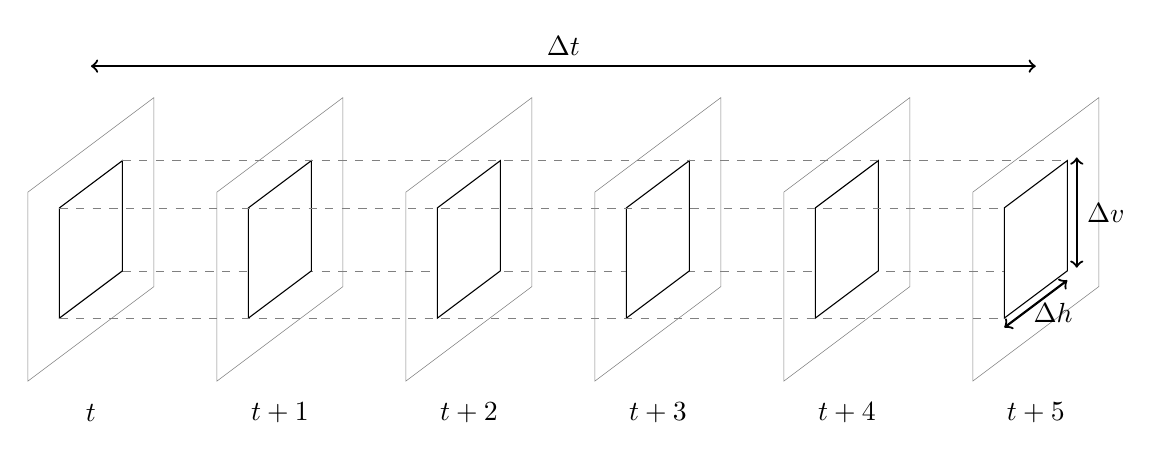
\begin{tikzpicture}[scale=0.4] % schéma du tube VQM dans une image

\draw[dashed,help lines] (3,3.5) -- (31,3.5);

\foreach \j in {0,3,6,9,12,15} % grille sur les autres images
{
	\draw[help lines] (2*\j,0) -- (4+2*\j,3) -- (4+2*\j,9) -- (2*\j,6) -- cycle;
	\filldraw[fill=white] (2*\j+1,2) -- (3+2*\j,3.5) -- (3+2*\j,7) -- (2*\j+1,5.5) -- cycle;
}

\path[thick,draw,<->] (33.3,3.6) -- (33.3,7.1) node[right,pos=0.5] {$\Delta v$};
\path[thick,draw,<->] (31,1.7) -- (33,3.2) node[right,pos=0.3] {$\Delta h$};
\path[thick,draw,<->] (2,10) -- (32,10) node[above,pos=0.5] {$\Delta t$};
\draw (2,-1) node{$t$};

\foreach \j in {1,2,3,4,5} % grille sur les autres images
{
	\draw (2+6*\j,-1) node{$t+\j$};
}

\draw[dashed,help lines] (1,5.5) -- (31,5.5);
\draw[dashed,help lines] (1,2) -- (31,2);
\draw[dashed,help lines] (3,7) -- (33,7);

\end{tikzpicture}
